% Part: sets-functions-relations
% Chapter: arithmetization
% Section:reals

\documentclass[../../../include/open-logic-section]{subfiles}

\begin{document}

\olfileid{sfr}{arith}{real}
\olsection{实数线}

下一步是展示如何从有理数构造实数。在此之前，我们需要理解实数究竟有什么\emph{独特性}。

实数的表现与有理数非常相似。（从技术上讲，两者都是\emph{有序域}的例子；关于其定义，参见\olref[check]{orderedfield}。）如果完成了\olref[sfr][siz][]{chap}的练习，就会知道实数严格多于有理数，即$\cardless{\Rat}{\Real}$。这是Cantor首先证明的。但人们知道存在无理数（即非有理数的实数）已有两千五百多年了。事实上：
%\footnote{Now: ``$\sqrt{2}$'' equally refers to both the positive and the negative roots; but in the next few pages, I'll forget about this, and consider only the positive root.}

\begin{thm}\ollabel{root2irrational}
$\sqrt{2}$ 不是有理数，即 $\sqrt{2} \notin \Rat$。
\end{thm}

\begin{proof}
反设$\sqrt{2}$是有理数。那么存在自然数$m$和$n$使得$\sqrt{2} =
\nicefrac{m}{n}$。事实上，我们可以选择$m$和$n$使得该分数不可再约分。整理得，$m^{2} = 2n^{2}$。由此，我们可以用两种方式完成证明：

\emph{其一，几何地}（遵循Tennenbaum）。\footnote{此证明由\cite{Conway2006}记载。}考虑以下正方形：
\begin{center}	
	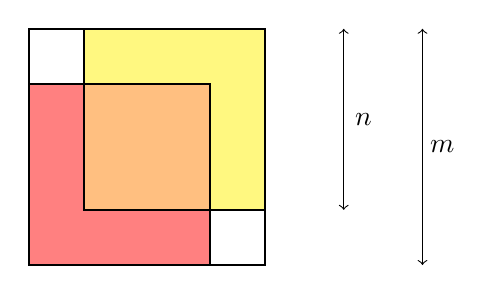
\begin{tikzpicture}
		\draw[thick] (0,0) rectangle (3,3);
		\draw[thick, fill=red!50] (0,0) rectangle (2.3,2.3);
		\draw[thick, fill=yellow!50] (0.7,0.7) rectangle (3, 3);
		\draw[thick, fill=orange!50] (0.7,0.7) rectangle (2.3, 2.3);
		\draw[<->] (4, 0.7)--(4, 3);
		\node at (4.25, 1.85) (n) {$n$};
		\draw[<->] (5, 0)--(5, 3);
		\node at (5.25, 1.5) (m) {$m$};
	\end{tikzpicture}
\end{center}
由于$m^2 = 2n^2$，两个边长为$n$的正方形重叠部分的面积，等于这两个正方形都未覆盖部分的面积；即橙色正方形的面积等于两个未着色正方形的面积之和。设橙色正方形边长为$p$，每个未着色正方形边长为$q$，则有$p^2 = 2q^2$。但现在$\sqrt{2} = \nicefrac{p}{q}$，其中$p < m$且$q < n$且$p, q \in \Nat$。这与$m$和$n$已被选为尽可能小相矛盾。
		
\emph{其二，形式地。}既然$m^{2} = 2n^{2}$，那么$m$是偶数。（容易证明，若$x$是奇数，则$x^2$是奇数。）所以存在某个$r \in \Nat$使得$m = 2r$。重新整理得$2r^2 = n^2$， 
		%				\begin{align*}
		%					(2q)^{2} &= 2n^{2}\\
		%					4q^{2} &= 2n^{2}\\
		%					2q^{2} &= n^{2}
		%				\end{align*}
于是$n$也是偶数。所以$m$和$n$都是偶数，因此分数$\nicefrac{m}{n}$\emph{可以}进一步约分。矛盾！
\end{proof}

顺带一提，借由这一图示证明，我们可以重温\olref[his][set][mythology]{sec}中的内容。Tennenbaum（1927--2006）是一位地道的现代数学家；但这个证明无疑十分优美，完全严谨，并且诉诸几何直觉！

不管怎样：实数比有理数“更广阔”。在某种意义上，有理数中存在“间隙”，而这些间隙被实数填补了。Weierstrass意识到，这刻画了实数的一个单一性质，正是该性质将实数与有理数区分开来，即完备性质：\emph{每个有上界的非空实数集都有一个最小上界。} 

容易看出有理数不具备完备性质。例如，考虑所有小于$\sqrt{2}$的有理数组成的集合，即：
\[
	\Setabs{p \in \Rat}{p^2 < 2 \text{ 或 }p < 0}
\]
这个集合在有理数中有上界；例如，它的所有元素都小于$3$。但它的最小上界是什么？我们想说“$\sqrt{2}$”；但我们刚刚看到$\sqrt{2}$\emph{不是}有理数。并且不存在大于$\sqrt{2}$的\emph{最小}有理数。所以该集合有上界但没有最小上界。因此有理数缺乏完备性质。

相比之下，连续统“理应”具有完备性质。我们不仅仅希望$\sqrt{2}$是一个实数；我们更希望填补有理数线上的所有“间隙”。事实上，我们希望连续统本身内部也不存在“间隙”。而这正是完备性将带给我们的。

\end{document}